\documentclass[a4]{article}

\usepackage[left=3cm,right=3cm,top=2cm,bottom=2cm]{geometry} 

\usepackage[utf8]{inputenc} 
\usepackage[           spanish % para poder usar el español
                      ,es-tabla % para los captions de las tablas
                       ]{babel}   
\decimalpoint

\usepackage[bookmarks=true,
            bookmarksnumbered=false, % true means bookmarks in 
                                     % left window are numbered
            bookmarksopen=false,     % true means only level 1
                                     % are displayed.
            colorlinks=true,
            linkcolor=blue,
            urlcolor=cyan]{hyperref}
            
\usepackage[T1]{fontenc}
\usepackage{lmodern}

\usepackage{parskip}
\usepackage{xcolor}

\usepackage{multirow}

\usepackage{amsmath,amssymb,amsthm}

\usepackage{caption}

\usepackage{listings}
\lstset
{ %Formatting for code in appendix
  language=C++, % choose the language of the code
  basicstyle=\fontfamily{pcr}\selectfont\footnotesize\color{black},
  keywordstyle=\color{darkorange}\bfseries, % style for keywords
  numbers=left, % where to put the line-numbers
  numberstyle=\tiny, % the size of the fonts that are used for the line-numbers     
  backgroundcolor=\color{white},
  showspaces=false, % show spaces adding particular underscores
  showstringspaces=false, % underline spaces within strings
  showtabs=false, % show tabs within strings adding particular underscores
  tabsize=2, % sets default tabsize to 2 spaces
  captionpos=b, % sets the caption-position to bottom
  breaklines=false, % sets automatic line breaking
  breakatwhitespace=false, 
}

\usepackage{enumerate}% paquete para poder personalizar fácilmente la apariencia de las listas enumerativas

\usepackage{graphicx} % figuras
\usepackage{subfigure} % subfiguras

\definecolor{darkorange}{rgb}{0.94,0.4,0.0}
	
\usepackage{float} % para controlar la situación de los entornos flotantes

\restylefloat{figure}
\restylefloat{table} 

\newcommand{\HRule}{\rule{\linewidth}{0.5mm}}

\author{David Cabezas Berrido\\ Patricia Córdoba Hidalgo\\ Emilio Hoyo Medina\\ Inmaculada Marín Carballo}
\date{\vspace{-5mm}}

\title{\huge Práctica 3: Algoritmos Greedy \HRule\vspace{-4mm}}

%\setcounter{section}{-1}

\begin{document}
\maketitle
\vspace{20mm}
\tableofcontents
\newpage

\section{Introducción}

El problema del viajante de comercio (TSP) consiste en encontrar el
ciclo hamiltoniano de peso mínimo en un grafo conexo y ponderado. En
esta práctica intentaremos abordar este problema por tres algoritmos
greedy distintos.

\subsection{Enfoque greedy}

Primero identificamos las características propias de un problema greedy:
\begin{enumerate}
\item \textbf{Conjunto de candidatos:} Las distintas ciudades a
  recorrer, que serán los nodos del grafo.
\item \textbf{Candidatos ya usados:} Ciudades ya añadidas al ciclo.
\item \textbf{Criterio solución:} Una permutación del conjunto de
  ciudades es solución.
\item \textbf{Criterio factible:} Cualquier lista de ciudades (no
  repetidas) puede llegar a ser solución.
\item \textbf{Función de selección:} A determinar por el algoritmo.
\item \textbf{Función objetivo:} A un ciclo solución le asocia la suma de los pesos de las aristas de dicho ciclo (debemos minimizarla).
\end{enumerate}

\section{Algoritmos}

\subsection{Algoritmo del vecino más cercano}

Se toma un vértice cualquiera y se añade al conjunto solución, nosotros
tomamos el primero. A continuación buscamos el vértice más cercano a
éste, y se añade también a la solución. Seguimos tomando el vértice
más cercano al último añadido que no esté en el conjunto
solución y repetimos el proceso hasta que todos los vértices estén en
el conjunto solución.

\subsubsection{Código}

\begin{lstlisting}
  vector<int> result(n);
  result[0] = 0;

  int dmin;
  int sumDistances=0;
  for(int k = 1; k < n; k++){
    dmin = INT_MAX;

    for(j = 0; j < n; j++)
      if(find(result.begin(),result.end(),j) == result.end()){
        distance = map[max(j,result[k-1])][min(j,result[k-1])];
        if(distance < dmin){
          i = j;
          dmin = distance;
        }
      }
    sumDistances += dmin;
    result[k] = i;
  }
  
  sumDistances += map[max(result[0],result[n-1])][min(result[0],result[n-1])];  
\end{lstlisting}

\newpage

\subsubsection{Eficiencia teórica}

El algoritmo está formado por dos bucles for anidados, ambos hacen n iteraciones. Dentro del primer bucle hay tres operaciones, en las líneas 7, 17 y 18, de eficiencia $O(1)$, las cuales despreciaremos para el cálculo de la eficiencia. Dentro del segundo bucle hay dos \verb-if-, que contienen operaciones de $O(1)$ también despreciables. En el primer \verb-if-, la condición (función find) tiene un eficiencia de $O(k)$, donde $k$, donde $k$ es el tamaño del vector solución. Por lo tanto la eficicencia total del algoritmo es:

$$n*\sum_{k=1}^{n}k = n*\frac{(n+1)*n}{2} = \frac{n^3+n^2}{2}$$

Luego el algoritmo es de $O(n^3)$

\subsubsection{Eficiencia empírica}

\begin{tabular}{|c|c|} \hline
\textbf{Tamaño}& 
\textbf{Algoritmo de cercanía}
  \\ \hline
     16      & 0.000129  \\
     22      & 0.000318  \\
     48      & 0.000712  \\
     70      & 0.002054  \\
     101     & 0.005609            \\
     150     & 0.016716  \\
     202     & 0.035437  \\
     280     & 0.086349    \\
     442     & 0.331839    \\
     561     & 0.671705  \\
     666     & 1.116590       \\
     1002    & 3.849760  \\
     2392    & 50.81290   \\
\hline
\end{tabular}

\vspace{5mm}
\textbf{Coeficientes del ajuste:}
\begin{verbatim}
Final set of parameters            Asymptotic Standard Error
=======================            ==========================

a               = 3.58701e-09      +/- 1.914e-11    (0.5336%)
b               = 3.55782e-07      +/- 6.155e-08    (17.3%)
c               = -0.000135481     +/- 4.139e-05    (30.55%)
d               = 0.00906667       +/- 0.005465     (60.28%)

rms of residuals      (FIT_STDFIT) = sqrt(WSSR/ndf)    : 0.00992738
variance of residuals (reduced chisquare) = WSSR/ndf   : 9.85529e-05
\end{verbatim}

\vspace{5mm}
Luego la gráfica que ajusta la función es:  $3.58701*10^{-9}x^3 + 3.55782*10^{-7}x^2 - 0.000135481x + 0.00906667$ 

\begin{figure}[H]
  \centering
\subfigure[Cercanía]{\label{graf:ulysses16}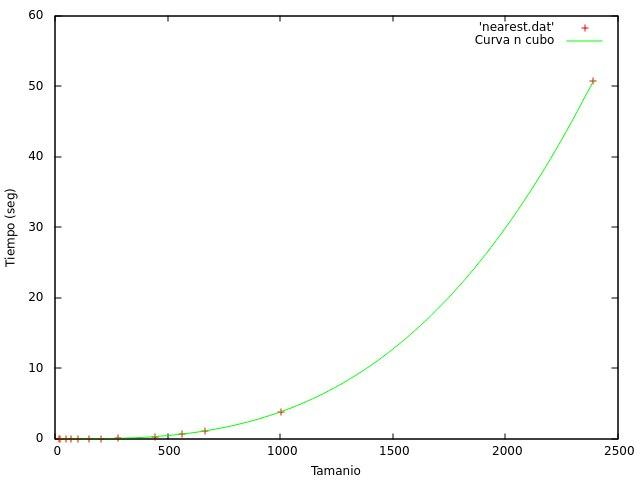
\includegraphics[width=100mm]{graficas/ajustes/nearest.jpg}}
\end{figure}

\subsection{Algoritmo de inserción}

Partimos de un recorrido parcial, que incluye la ciudad más al norte,
la ciudad más al este y más al oeste. A continuación, buscamos la
ciudad (entre los candidatos sin escoger) y la posición (en el ciclo)
que supongan un menor incremento en el peso del ciclo y añadimos dicha
ciudad en esa posición. Repetimos este proceso hasta que todos los
vértices estén en el conjunto solución.

\subsubsection{Código}

\begin{lstlisting}
  int sumDistances=0;
  vector<int> result(3);

  //Incluimos las tres ciudades iniciales 
  result[0]=maxX;
  result[1]=minX;
  result[2]=maxY;

  //Sumo las distancias de las 3 ciudades entre ellas
  sumDistances += map[max(result[1],result[0])][min(result[1],result[0])];
  sumDistances += map[max(result[2],result[0])][min(result[2],result[0])];
  sumDistances += map[max(result[1],result[2])][min(result[1],result[2])];

  //Creo un vector con las ciudades que quedan por recorrer (borro las 3 ya escogidas)
  vector<int> candidates(n);
  for(i = 0; i < n; i++) candidates[i]=i;
  candidates.erase(remove(candidates.begin(),candidates.end(),maxX));
  candidates.erase(remove(candidates.begin(),candidates.end(),minX));
  candidates.erase(remove(candidates.begin(),candidates.end(),maxY));
  
  int bestCity;
  int bestPosition;
  int bestD;
  int d;

  while(candidates.size()>0){ // Mientras que queden candidatos (ciudades sin recorrer)
    for(i = 0; i < candidates.size(); i++){
      bestD = INT_MAX;
      for(j = 0; j < result.size(); j++){ // Miro cual es el incrementodel peso que supone insertar esa ciudad en cada posible posicion
        d = map[max(result[j],candidates[i])][min(result[j],candidates[i])]
        + map[max(result[(j+1)%result.size()],candidates[i])]
             [min(result[(j+1)%result.size()],candidates[i])]
        - map[max(result[(j+1)%result.size()],result[j])]
             [min(result[(j+1)%result.size()],result[j])];
        if(d < bestD){ //Buscamos la ciudad y la posicion que minimicen el incremento de la distancia
          bestCity = candidates[i];
          bestPosition = (j+1)%result.size();
          bestD = d;
        }
      }
    }
    result.insert(next(result.begin(),bestPosition),bestCity); //inserto la ciudad en el vector de resultados
    candidates.erase(remove(candidates.begin(),candidates.end(),bestCity)); //borro la ciudad del vector de candidatos
    sumDistances += bestD; //Sumo la distancia a la distancia total del recorrido
  }
\end{lstlisting}

\subsubsection{Eficiencia teórica}

Calculemos la eficiencia teórica del algoritmo de inserción para el
problema del viajante de comercio. Sea n el número de ciudades. Como
vemos tenemos un bucle externo en el cuál en cada iteración se escoge
la siguiente ciudad del recorrido. Este bucle se ejecuta hasta que
todas las ciudades estén en el recorrido, es decir, se ejecuta n-3
veces. Podemos suponer que se ejecuta n veces. Supongamos que k es el
tamaño del vector de ciudades que todavía no están en el
recorrido. Por tanto, el bucle intermedio se ejecutaría k veces con k
variando entre n y 0 (k va decreciendo en cada iteración del bucle
externo), y el bucle interno se ejecuta n-k veces, pues se ejecuta
tantas veces como ciudades ya hayamos metido en el recorrido. El
interior del bucle interno es O(1). El interior del bucle interno
tiene eficiencia O(n). Además, las operaciones de borrado e inserción
al final del bucle externo tienen eficiencia O(n). Por tanto
tendríamos la siguiente sumatoria:

\begin{align*}
\sum_{k=1}^{n}(k((n-k)+1)+n)&=\sum_{k=1}^{n}kn-\sum_{k=1}^{n}k^2+\sum_{k=1}^{n}k+\sum_{k=1}^{n}n\\&=n(\frac{n(n+1)}{2})-\frac{n(n+1)(2n+1)}{6}+\frac{n(n+1)}{2}+n^2\\&=\frac{3n^3+3n^2}{6}-\frac{2n^3+3n^2+n}{6}+\frac{n(n+1)}{2}+n^2\\&=\frac{n^3-n}{6}+\frac{n(n+1)}{2}+n^2
\end{align*}
Y por lo tanto la eficiencia teórica del algoritmo es $O(n^3)$.

\subsubsection{Eficiencia empírica}

\begin{tabular}{|c|c|} \hline
\textbf{Tamaño}& 
\textbf{Algoritmo de inserción}
  \\ \hline
     16      & 0.000285  \\
     22      & 0.000702  \\
     48      & 0.002520  \\
     70      & 0.006446  \\
     101     & 0.019039            \\
     150     & 0.054795  \\
     202     & 0.121605  \\
     280     & 0.314127    \\
     442     & 1.295430    \\
     561     & 2.619400  \\
     666     & 4.445740       \\
     1002    & 15.04680  \\
     2392    & 217.6250   \\
\hline
\end{tabular}

\newpage
\textbf{Coeficientes del ajuste:}
\begin{verbatim}
Final set of parameters            Asymptotic Standard Error
=======================            ==========================

a               = 1.69297e-08      +/- 1.007e-10    (0.5945%)
b               = -2.87207e-06     +/- 3.237e-07    (11.27%)
c               = 0.00100639       +/- 0.0002177    (21.63%)
d               = -0.0541579       +/- 0.02874      (53.07%)

rms of residuals      (FIT_STDFIT) = sqrt(WSSR/ndf)    : 0.0522078
variance of residuals (reduced chisquare) = WSSR/ndf   : 0.00272565
\end{verbatim}

Luego la gráfica que ajusta la función es: $1.69297*10^{-8}x^3 - 2.87207*10^{-6}x^2 + 0.00100639x - 0.0541579$ 

\begin{figure}[H]
  \centering
\subfigure[Inserción]{\label{graf:ulysses16}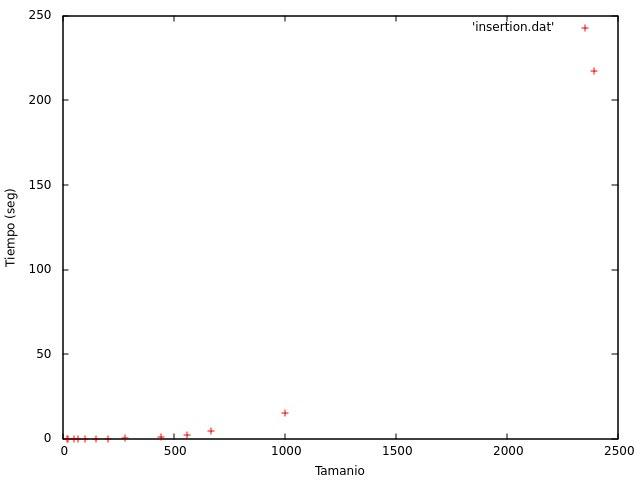
\includegraphics[width=100mm]{graficas/ajustes/insertion.jpg}}
\end{figure}

\subsection{Nuestra propuesta: Algoritmo double nearest}

Nuestro algortimo busca cuales son las dos cuidades cuya suma de sus
distancias es la mínima respecto a la última ciudad recorrida, por los que se seleccionan dos ciudades cada vez, gracias a tres bucles
anidados.

Se va rellenando en el vector de resultados con las ciudades con
distancias más óptimas, y sumando el total de las distancias
calculadas. Una vez se ha hecho esto, en cada iteración se borran las
ciudades de los candidatos a recorrer, ya que no volveremos a pasar
por ellas.

Para decidir que ciudades son las optimas, para cada ciudad
candidata se calcula la distancia entre ella y todas las demás ciudades, buscando el camino más optimo hacia cualquiera del resto de candidatos. Así escogemos las dos ciudades óptimas.

Al salir de nuestro bucle anidado, si el numero de ciudades no era
par, asignamos al último elemento del vector de resultados nuestra
última ciudad candidata y sumamos la distancia de ésta a la anterior
cuidad.  Para finalizar, añadimos al recorrido total la distancia de
nuestra ultimo ciudad del camino a nuestra cuidad de origen. Ya
tendríamos nuestro circuito óptimo.

\newpage

\subsubsection{Código}

\begin{lstlisting}
vector<int> result(n);
result[0]=0;

vector<int> candidates(n-1);

for(i = 1; i < n; i++) candidates[i-1]=i;

int sumDistances=0, d1, d2, bestD, bestCity1, bestCity2;

for(int k = 1; k < (n+1)/2; k++){ // Relleno el vector result
  bestD = INT_MAX;
  for(i = 0; i < candidates.size(); i++){ // Para cada candidato
    d1 = map[max(candidates[i],result[2*k-2])][min(candidates[i],result[2*k-2])];
    d2 = INT_MAX;
    for(j = 0; j < candidates.size(); j++){ // Para el resto de candidatos
      if(candidates[j] != candidates[i]){
        d2 = map[max(candidates[i],candidates[j])][min(candidates[i],candidates[j])];
        if(d1 + d2 < bestD){
          bestD = d1 + d2;
          bestCity1 = candidates[i];
          bestCity2 = candidates[j];
	}
      }
    }
  }
  result[2*k-1] = bestCity1;
  result[2*k] = bestCity2;
  sumDistances += bestD;
  candidates.erase(remove(candidates.begin(),candidates.end(),bestCity1));
  candidates.erase(remove(candidates.begin(),candidates.end(),bestCity2));
}

if(!(n%2)){
  result[n-1] = candidates[0];
  sumDistances += map[max(result[n-1],result[n-2])][min(result[n-1],result[n-2])];
}

sumDistances += map[max(result[n-1],result[0])][min(result[n-1],result[0])];
\end{lstlisting}

\subsubsection{Eficiencia teórica}
Veamos la eficiencia teórica del algoritmo que hemos ideado
nosotros. Como vemos, el bucle externo del algoritmo se ejecuta n/2
veces. Los dos bucles internos se ejecutarían n-2k
(=candidates.size()) veces cada uno, siendo 2k el número de ciudades
que ya hemos añadido al recorrido (k es el índice por el que va el
bucle externo). Dado que están anidados uno dentro del otro estos se
ejecutan en total $(n-2k)^2$ veces. Las funciones erase y remove son
O(candidates.size())=O(n-2k). Por tanto, tenemos para calcular la
eficiencia teórica la siguiente sumatoria (con j=n/2):

  \begin{align*}
  \sum_{k=1}^{\frac{n}{2}}[(n-2k)^2+n-2k] &=\sum_{k=1}^j[n^2+4k^2-4nk+n-2k]\\&=jn^2+4\frac{j(j+1)(2j+1)}{6}-4n\frac{j(j+1)}{2}+jn-2\frac{j(j+1)}{2}\\&=\frac{n^3}{2}+4\frac{\frac{n^3}{2}+\frac{n^2}{2}+n^2+n}{12}-\frac{n^3}{2}-n^2+\frac{n^2}{2}-\frac{\frac{n^2}{2}+n}{2}\\&=\frac{n^3}{2}+\frac{n^3}{6}+\frac{n^2}{6}+\frac{n^2}{3}+\frac{n}{3}-\frac{n^3}{2}-\frac{n^2}{2}-\frac{n^2}{4}-\frac{n}{2}\\&=\frac{n^3}{6}+\frac{n^2}{6}+\frac{n^2}{3}+\frac{n}{3}-n^2-\frac{n^2}{2}-\frac{n^2}{4}-\frac{n}{2}
  \end{align*}
  Eficiencia: $O(n^3)$.

\subsubsection{Eficiencia empírica}

\begin{tabular}{|c|c|} \hline
\textbf{Tamaño}& 
\textbf{Algoritmo double nearest}
  \\ \hline
     16      & 9.1e-05   \\
     22      & 0.000288  \\
     48      & 0.001181  \\
     70      & 0.001640  \\
     101     & 0.005582            \\
     150     & 0.015294  \\
     202     & 0.031035  \\
     280     & 0.079450    \\
     442     & 0.309697    \\
     561     & 0.655716  \\
     666     & 1.102970       \\
     1002    & 3.842490  \\
     2392    & 57.64050   \\
\hline
\end{tabular}

\vspace{5mm}
\textbf{Coeficientes del ajuste:}
\begin{verbatim}
Final set of parameters            Asymptotic Standard Error
=======================            ==========================

a               = 4.61334e-09      +/- 2.595e-11    (0.5626%)
b               = -1.09743e-06     +/- 8.346e-08    (7.605%)
c               = 0.000332856      +/- 5.612e-05    (16.86%)
d               = -0.0161545       +/- 0.007411     (45.87%)

rms of residuals      (FIT_STDFIT) = sqrt(WSSR/ndf)    : 0.0134615
variance of residuals (reduced chisquare) = WSSR/ndf   : 0.000181212
\end{verbatim}

Luego la gráfica que ajusta la función es: $4.61334*10^{-9}x^3 - 1.09743*10^{-6}x^2 + 0.000332856x - 0.0161545 $ 

\begin{figure}[H]
  \centering
\subfigure[Double nearest]{\label{graf:ulysses16}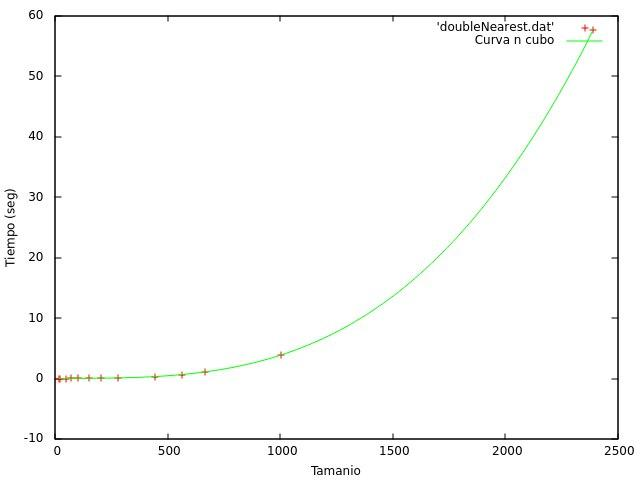
\includegraphics[width=100mm]{graficas/ajustes/doubleNearest.jpg}}
\end{figure}

\section{Resultados}

A continuación mostramos los ciclos obtenidos por los distintos
algoritmos en una serie de ejemplos y el peso de estos ciclos.

\subsection{ulysses16}

\begin{figure}[H]
  \centering
\subfigure[Ciudades]{\label{graf:ulysses16}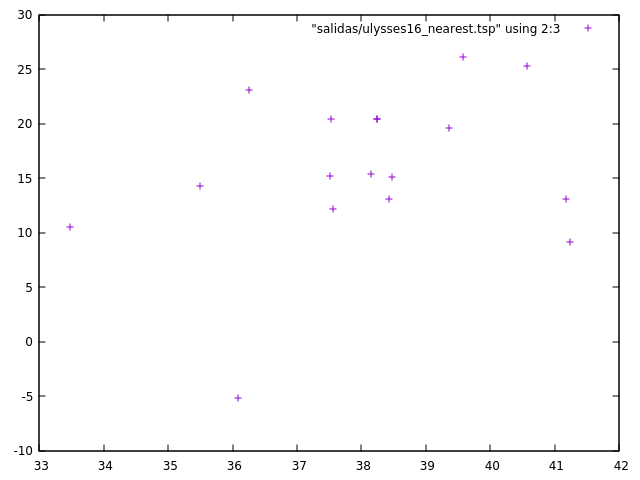
\includegraphics[width=55mm]{graficas/ulysses16}}
\subfigure[Algoritmo de cercanía. Peso = 103]{\label{graf:ulysses16_nearest}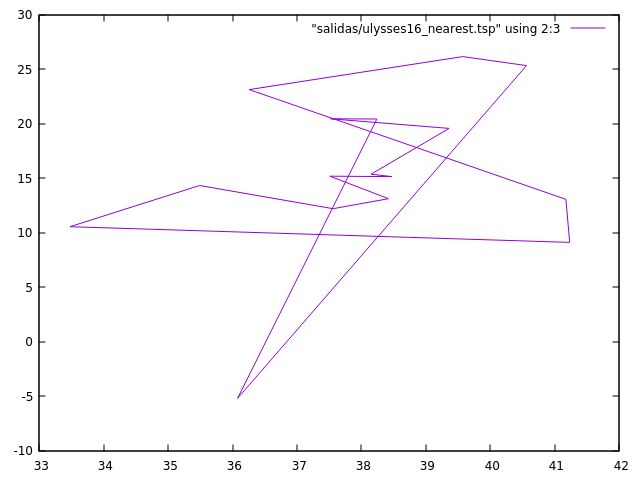
\includegraphics[width=55mm]{graficas/ulysses16_nearest}}
\subfigure[Algoritmo de inserción. Peso = 72]{\label{graf:ulysses16_insertion}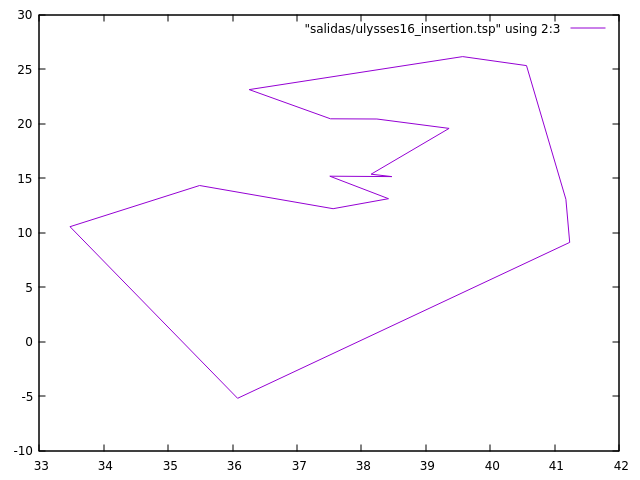
\includegraphics[width=55mm]{graficas/ulysses16_insertion}}
\subfigure[Algoritmo doubleNearest. Peso = 101]{\label{graf:ulysses16_...}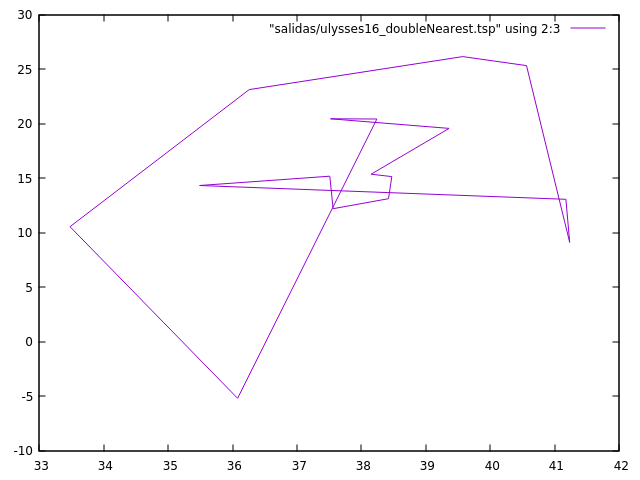
\includegraphics[width=55mm]{graficas/ulysses16_doubleNearest}}
\end{figure}

\subsection{st70}
\setcounter{subfigure}{0}

\begin{figure}[H]
  \centering
\subfigure[Ciudades]{\label{graf:st70}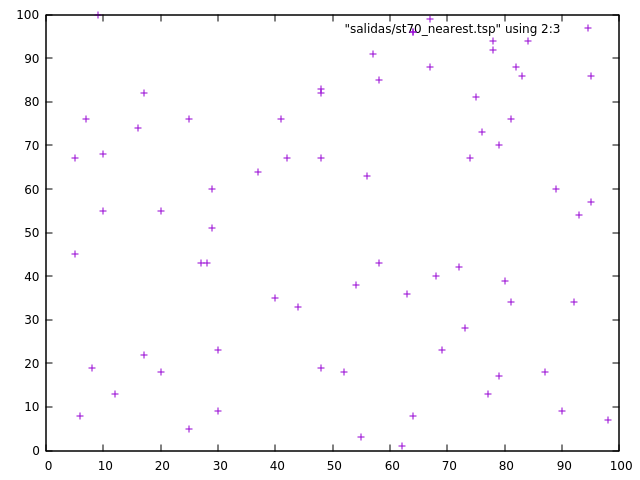
\includegraphics[width=55mm]{graficas/st70}}
\subfigure[Algoritmo de cercanía. Peso = 830]{\label{graf:st70_nearest}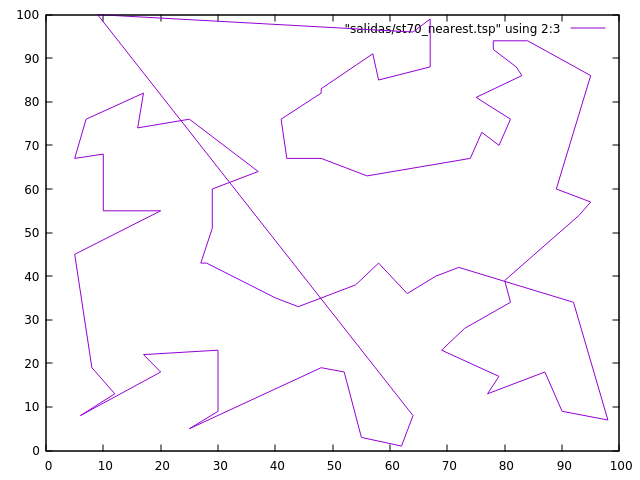
\includegraphics[width=55mm]{graficas/st70_nearest}}
\subfigure[Algoritmo de inserción. Peso = 754]{\label{graf:st70_insertion}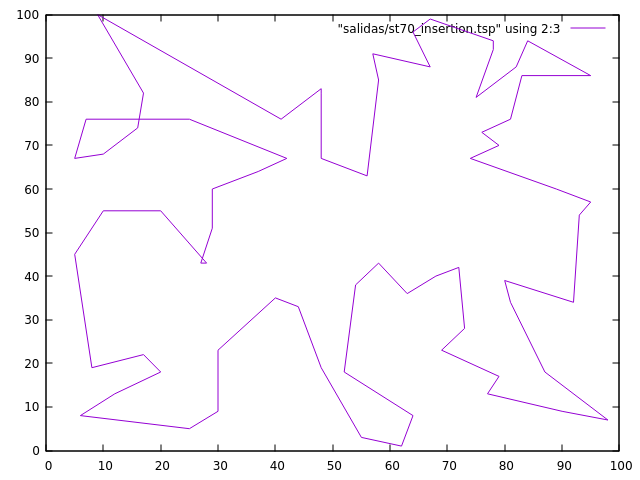
\includegraphics[width=55mm]{graficas/st70_insertion}}
\subfigure[Algoritmo doubleNearest. Peso = 958]{\label{graf:st70_...}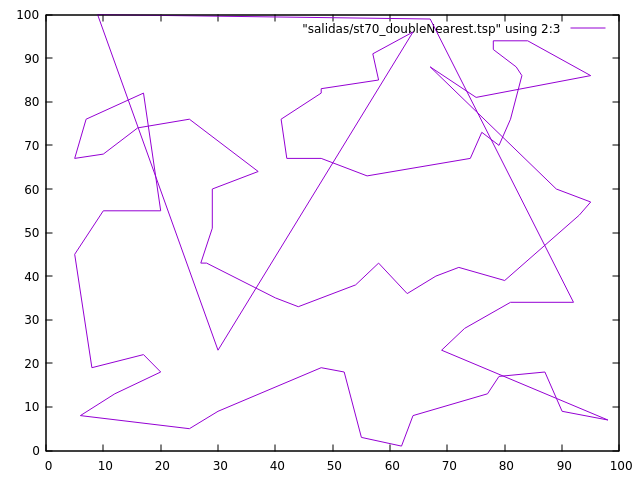
\includegraphics[width=55mm]{graficas/st70_doubleNearest}}
\end{figure}

\subsection{gr202}
\setcounter{subfigure}{0}

\begin{figure}[H]
  \centering
\subfigure[Ciudades]{\label{graf:gr202}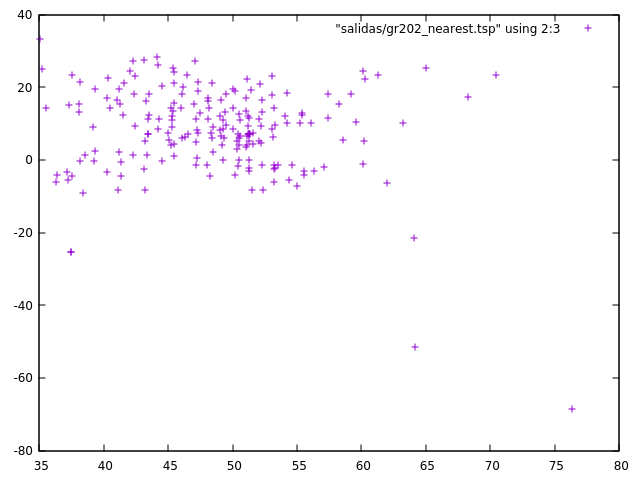
\includegraphics[width=55mm]{graficas/gr202}}
\subfigure[Algoritmo de cercanía. Peso = 651]{\label{graf:gr202_nearest}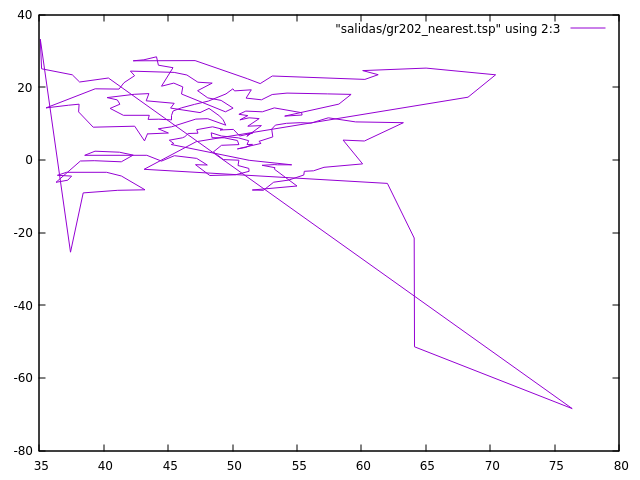
\includegraphics[width=55mm]{graficas/gr202_nearest}}
\subfigure[Algoritmo de inserción. Peso = 554]{\label{graf:gr202_insertion}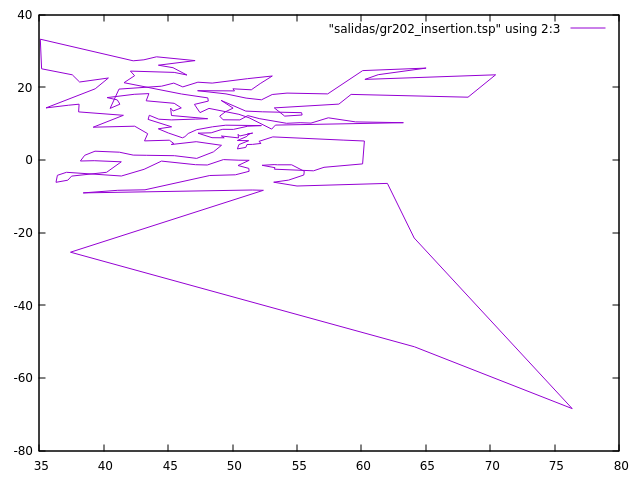
\includegraphics[width=55mm]{graficas/gr202_insertion}}
\subfigure[Algoritmo doubleNearest. Peso = 688]{\label{graf:gr202_...}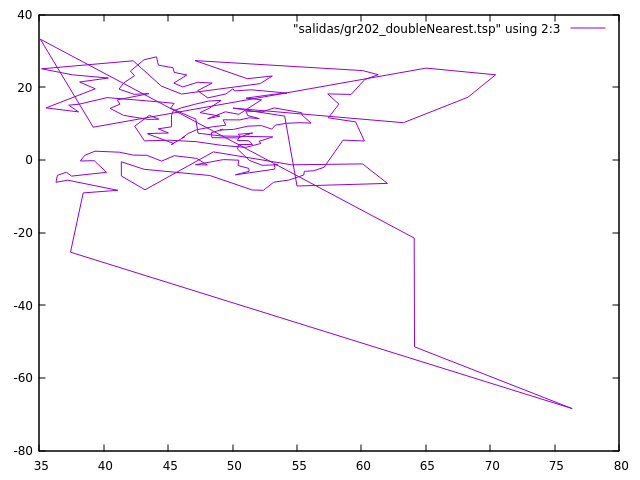
\includegraphics[width=55mm]{graficas/gr202_doubleNearest}}
\end{figure}

\subsection{gr666}
\setcounter{subfigure}{0}

\begin{figure}[H]
  \centering
\subfigure[Ciudades]{\label{graf:gr666}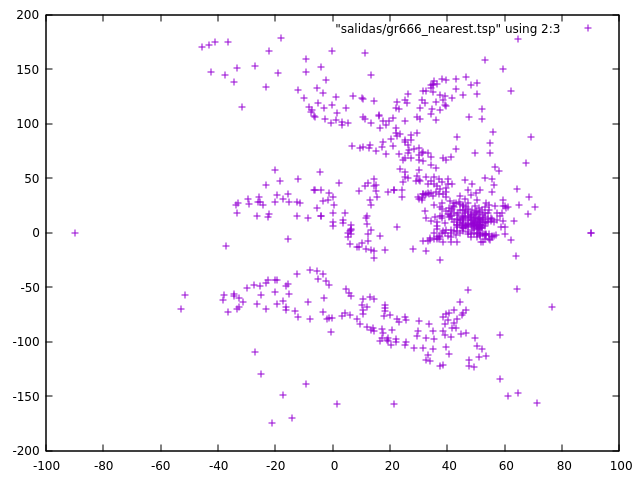
\includegraphics[width=55mm]{graficas/gr666}}
\subfigure[Algoritmo de cercanía. Peso = 4046]{\label{graf:gr666_nearest}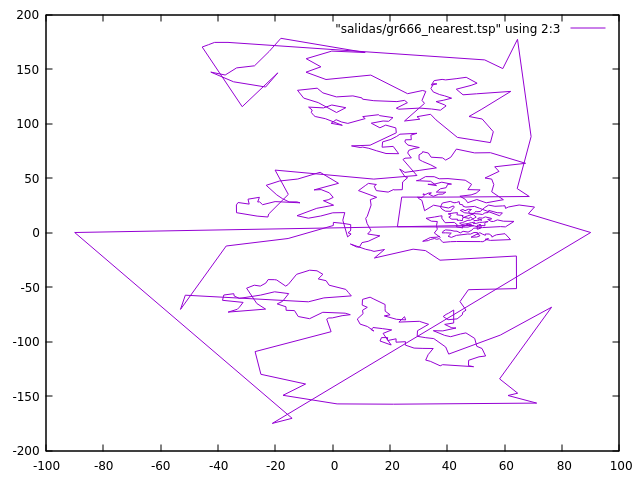
\includegraphics[width=55mm]{graficas/gr666_nearest}}
\subfigure[Algoritmo de inserción. Peso = 3656]{\label{graf:gr666_insertion}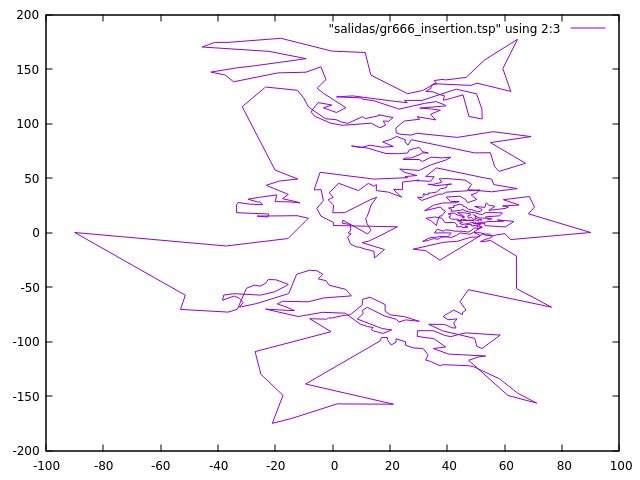
\includegraphics[width=55mm]{graficas/gr666_insertion}}
\subfigure[Algoritmo doubleNearest. Peso = 4452]{\label{graf:gr666_...}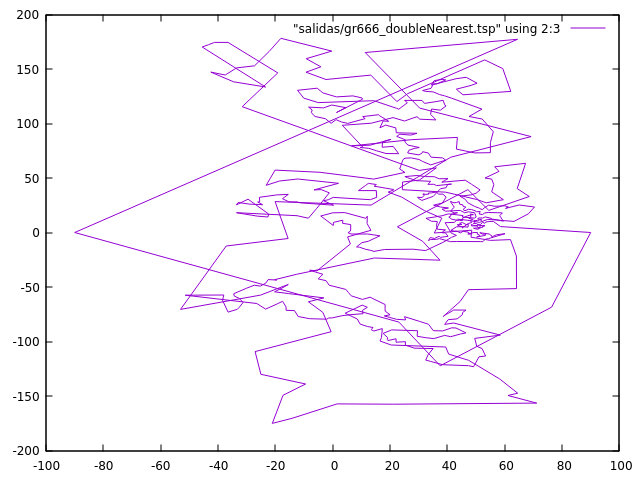
\includegraphics[width=55mm]{graficas/gr666_doubleNearest}}
\end{figure}

\subsection{pr1002}
\setcounter{subfigure}{0}

\begin{figure}[H]
  \centering
\subfigure[Ciudades]{\label{graf:pr1002}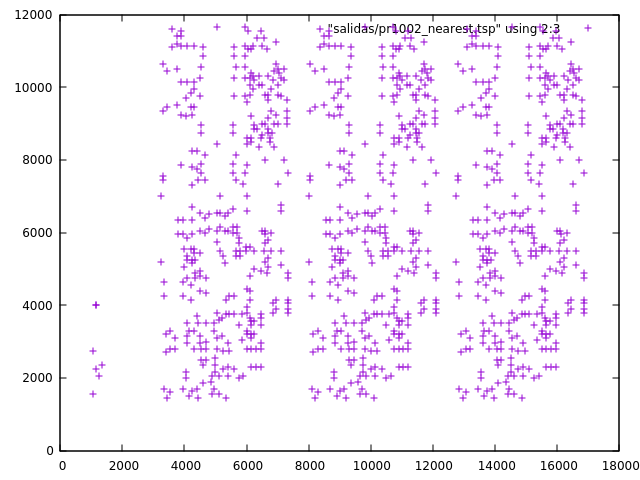
\includegraphics[width=55mm]{graficas/pr1002}}
\subfigure[Algoritmo de cercanía. Peso = 331103]{\label{graf:pr1002_nearest}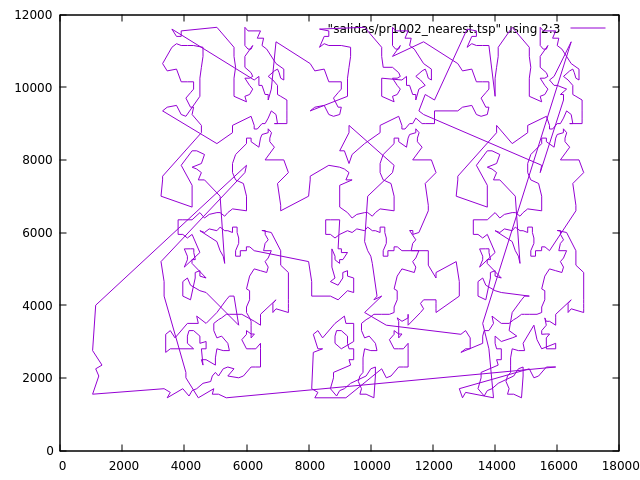
\includegraphics[width=55mm]{graficas/pr1002_nearest}}
\subfigure[Algoritmo de inserción. Peso = 316968]{\label{graf:pr1002_insertion}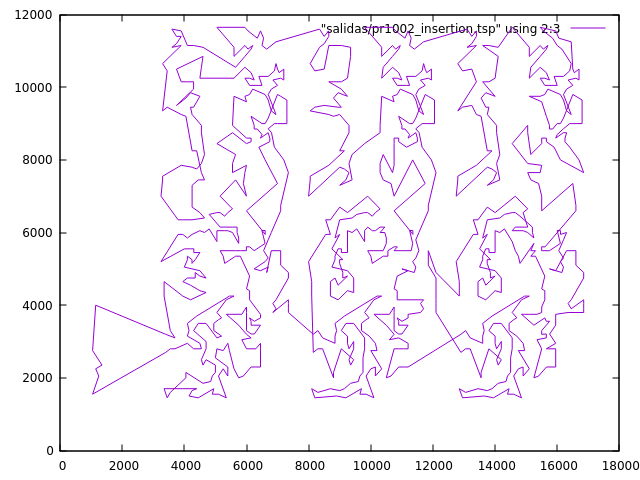
\includegraphics[width=55mm]{graficas/pr1002_insertion}}
\subfigure[Algoritmo doubleNearest. Peso = 385020]{\label{graf:pr1002_...}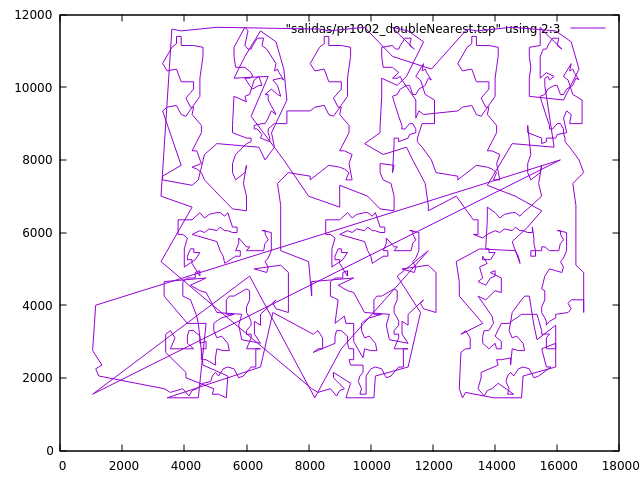
\includegraphics[width=55mm]{graficas/pr1002_doubleNearest}}
\end{figure}

\section{Conclusión}

A pesar de que los tres tienen el mismo orden de eficiencia, los
resultados que dan son diferentes.

En cuanto a tiempo, el algoritmo más rápido es el primero, el del
vecino más cercano. Le sigue nuestro algoritmo y el más lento es el de
inserción.

En cuanto a la solución óptima, el algoritmo de inserción es el que da
una mejor solución, en todos los casos la suma de los pesos es menor a
los demaś. El algoritmo de cercanía es el segundo que mejor soluciona
el problema. Nuestro algoritmo es el peor.

\begin{figure}[H]
  \centering
\subfigure[Comparación de tiempos]{\label{ef:comparison}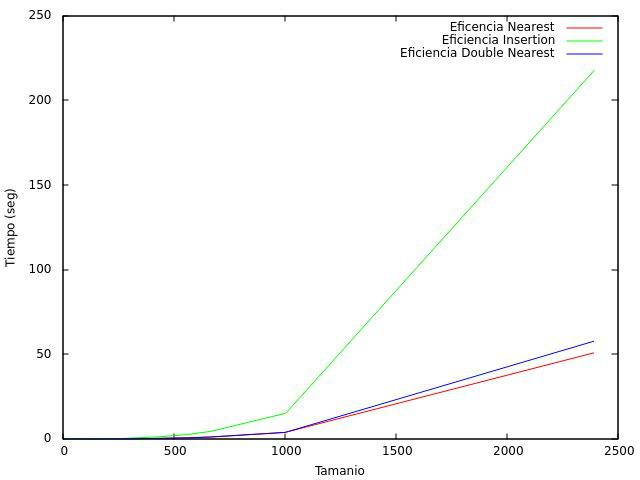
\includegraphics[width=100mm]{graficas/ajustes/comparison}}
\end{figure}

\end{document}